\documentclass{article}
\usepackage{amsmath, amssymb, kotex, hyperref, graphicx, mdframed, setspace,enumitem}
\usepackage[a4paper, margin = 40pt]{geometry}
\setstretch{1.5}
\newcommand\ar{\ensuremath{\text{AR}}}
\newcommand\ma{\ensuremath{\text{MA}}}
\newcommand\arma{\ensuremath{\text{ARMA}}}
\newcommand\cov{\ensuremath{\text{Cov}}}
\newcommand\sa{\ensuremath{{\sigma_a}^2}}

\begin{document}
\title{Arima Model - 5}
\author{강의 : 김성범 교수님\\ 정리 :  김선중}
\date{\today}
\maketitle

이것은 \href{https://youtu.be/K7GWJ3iC6OY}{ARIMA 모델 개요 - Part 5} 강의에 대한 노트이다.
이전과는 다르게 영어로 작성해보았다.
\tableofcontents

\newpage
\begin{center}
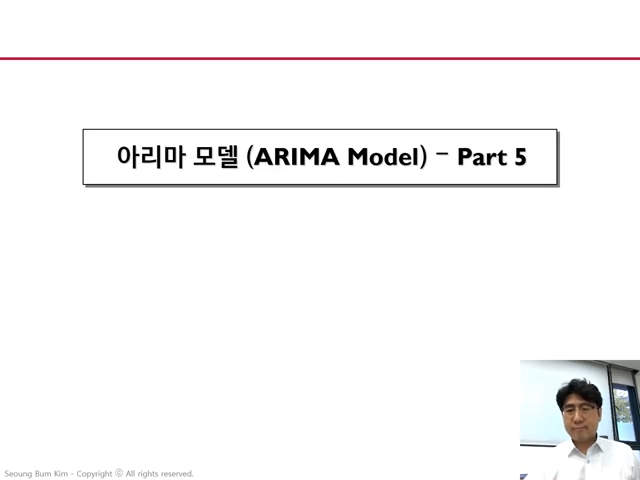
\includegraphics[width=.45\textwidth]{capture1}
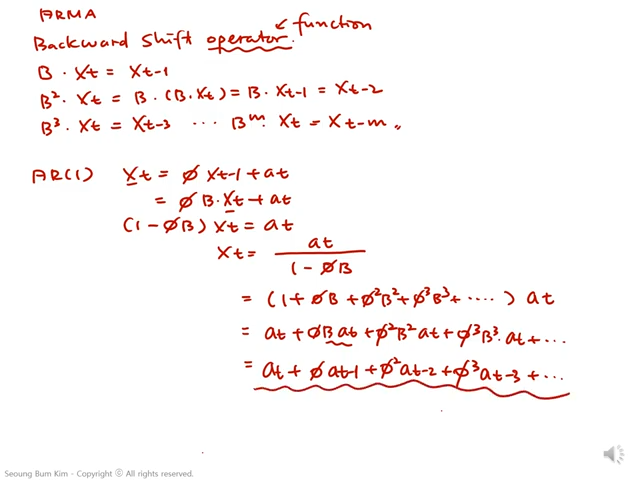
\includegraphics[width=.45\textwidth]{capture2}
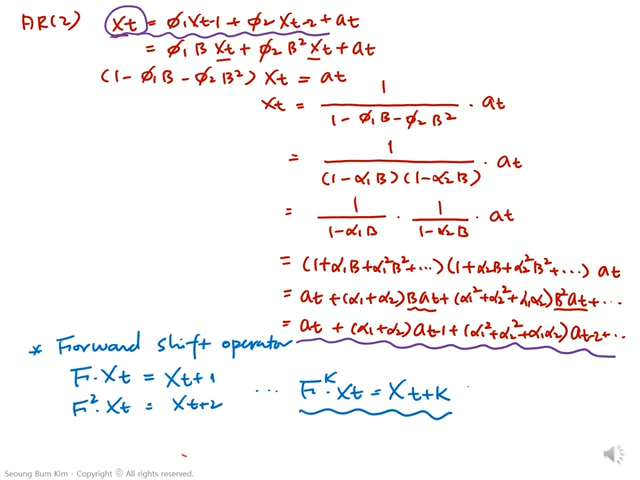
\includegraphics[width=.45\textwidth]{capture3}
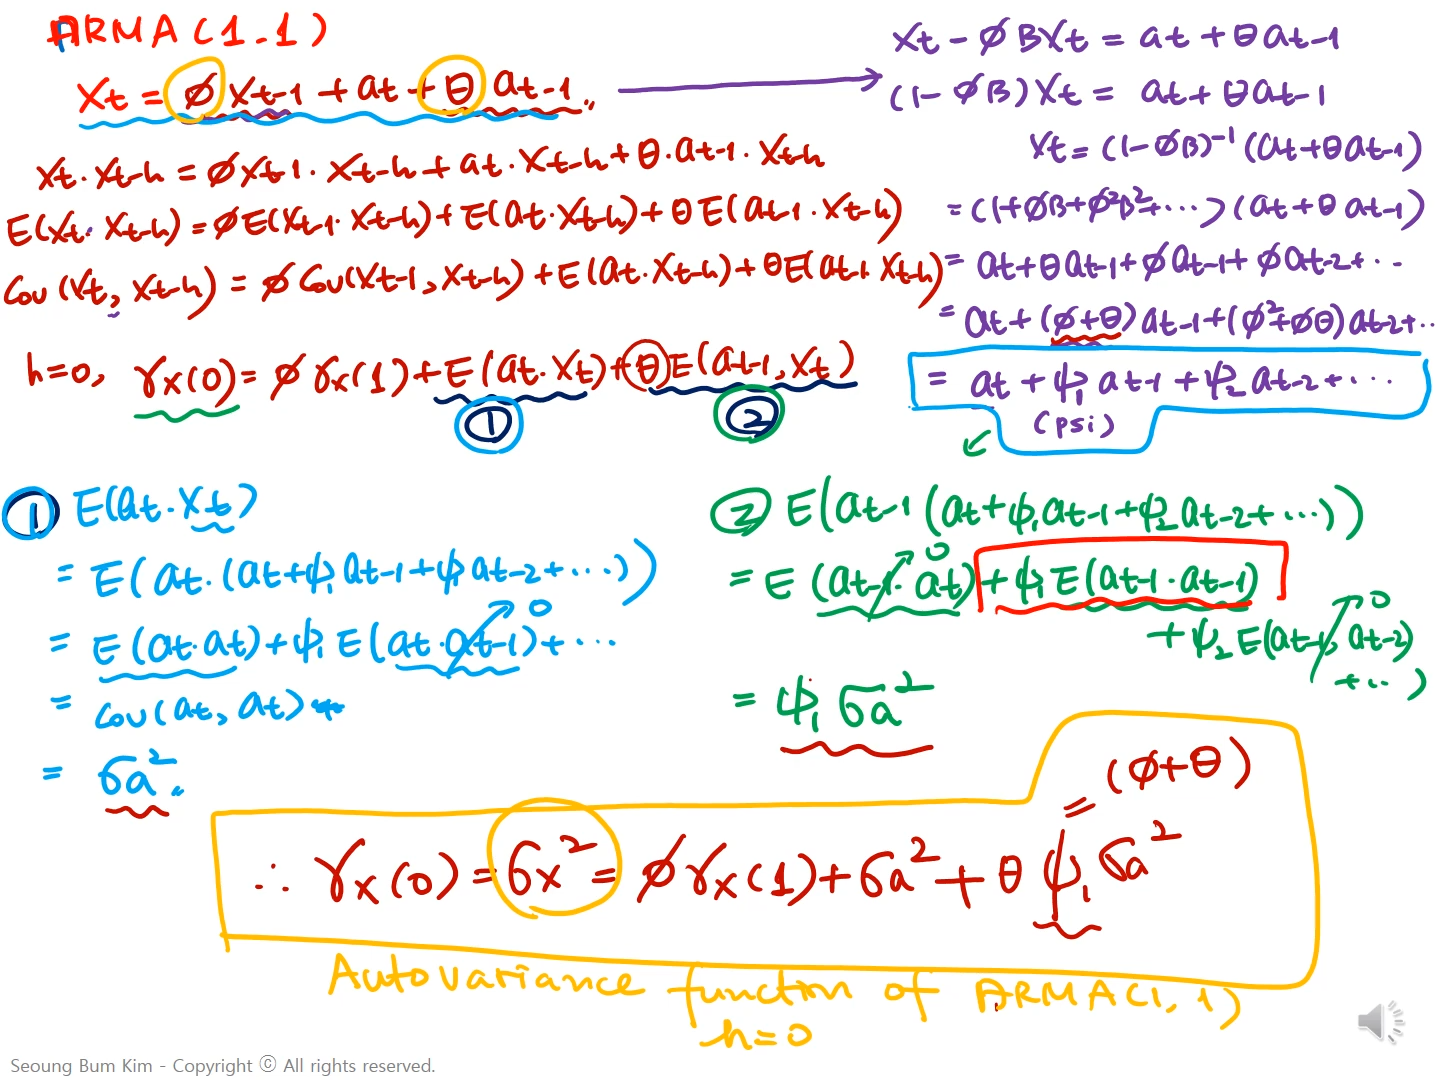
\includegraphics[width=.45\textwidth]{capture4}
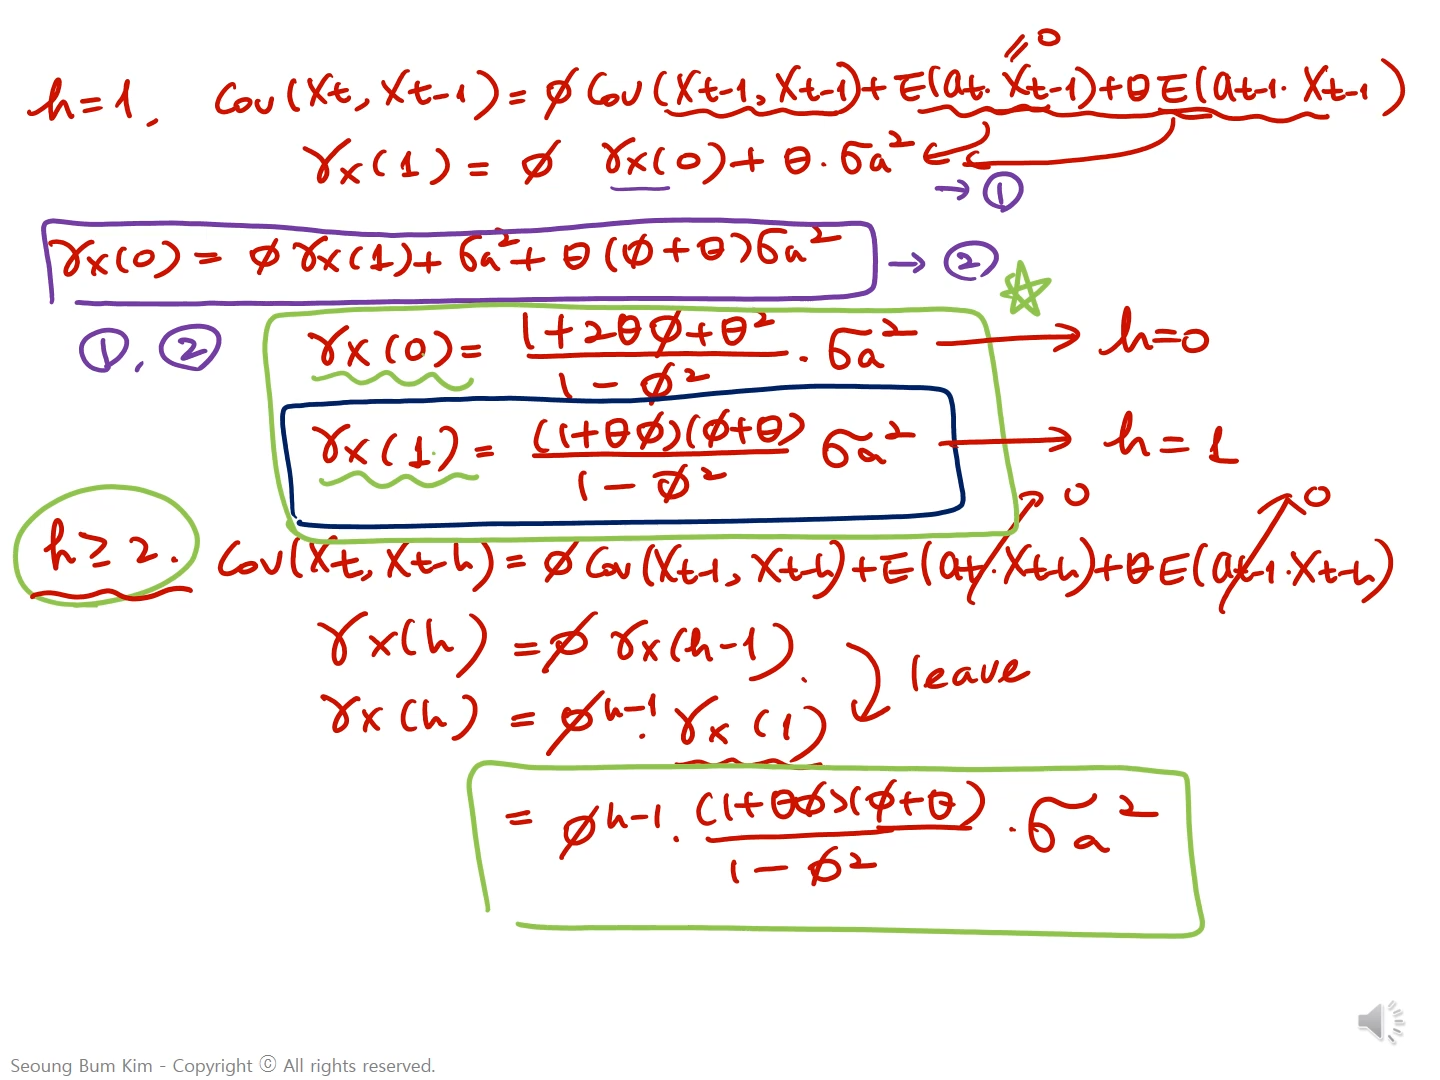
\includegraphics[width=.45\textwidth]{capture5}
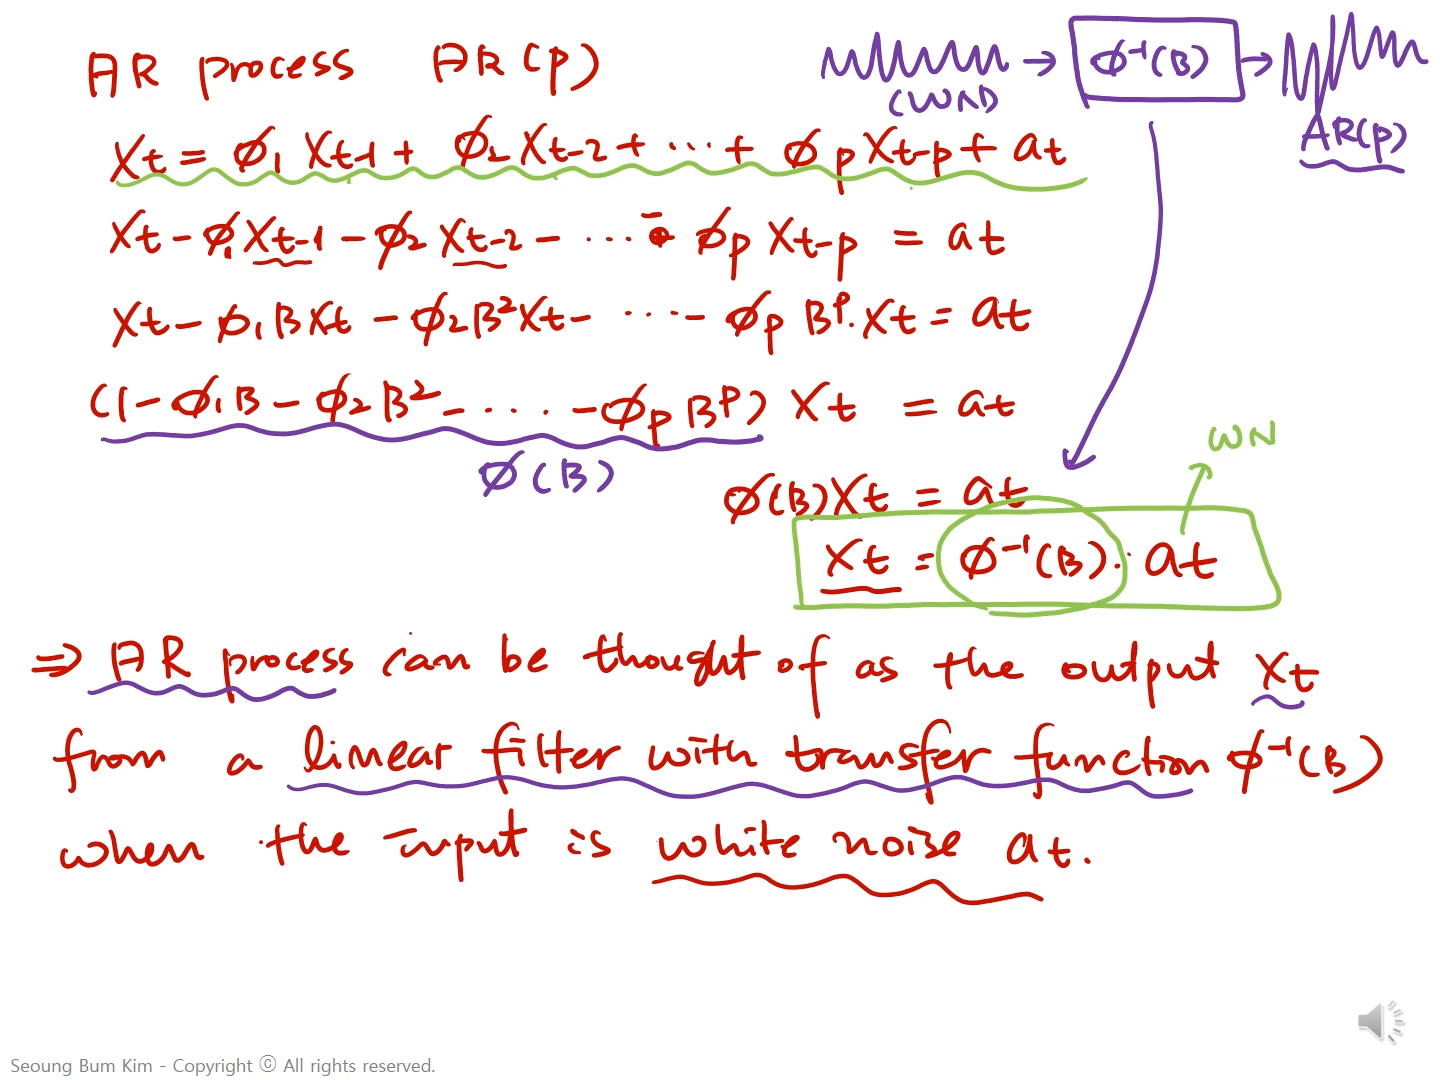
\includegraphics[width=.45\textwidth]{capture6}
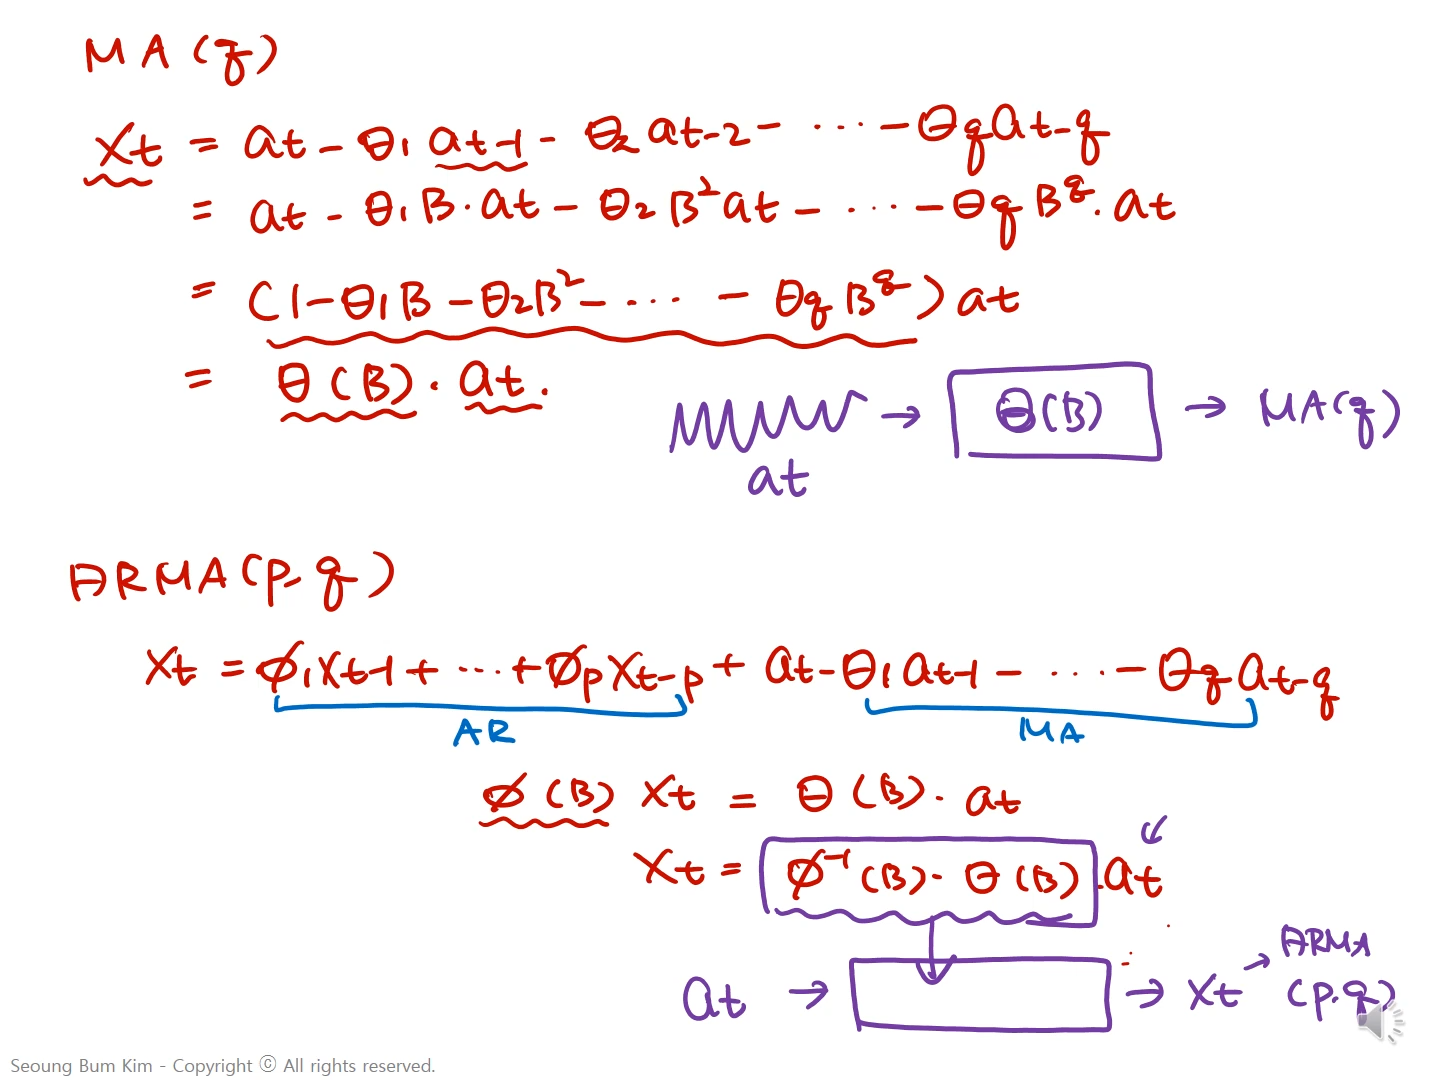
\includegraphics[width=.45\textwidth]{capture7}
\end{center}

%%
\section{Backward shift operator \(B\)}
An operator \(B\) is called the \emph{backward shift operator}.
It is a function that maps a random variable which depends on time (i.e. \(X_t\) or \(a_t\)), backward by one step.
\begin{equation}\label{bso}
B(X_t)=X_{t-1}
\end{equation}
We occasionally write \(B X_t\) instead of \(B(X_t)\) to stand for the same thing.
Denoting \(B^m=B\circ B\circ\cdots\circ B\) by the \(m\) times composition of \(B\), we have
\begin{align*}
B X_t &= X_{t-1}\\
B^2 X_t &= X_{t-2}\\
&\vdots\\
B^m X_t&=X_{t-m}.
\end{align*}
The professor tries to explain \ar(1) model and \ar(2) model in terms of this operator \(B\), which is illustrated as follows.

%
\subsection{AR(1) model described by \(B\)}
Recall that \ar(1) is called the \emph{autoregressive model} of order 1, which predict \(X_t\) by means of \(X_{t-1}\) and \(a_t\).
\begin{equation}\label{ar1}
X_t=\phi X_{t-1}+a_t.
\end{equation}
Here, \(a_t\) is a white noise so that the expectation of \(a_t\) is 0 ;
\begin{equation}\label{white_noise_1}
\mathbb E[a_t]=0,
\end{equation}
the variance of \(a_t\) is independent of \(t\) ;
\begin{equation}\label{white_noise_2}
\mathbb V[a_t]=\sa,
\end{equation}
and \(a_t\)'s in distinct timsteps are independent one another ;
\begin{equation}\label{white_noise_3}
\cov(a_t,a_{t+h})=0\quad\text{for}\quad h\neq0.
\end{equation}
Recall that \(\mathbb V[X]=\mathbb E[X^2]-(\mathbb E[X])^2\) for any random variable \(X\).
By \eqref{white_noise_1} and \eqref{white_noise_2},
\begin{equation}\label{white_noise_4}
\mathbb E[{a_t}^2]=\mathbb V[a_t]+(\mathbb E[a_t])^2=\sa+0^2=\sa.
\end{equation}
Moreover, by \eqref{white_noise_1} and \eqref{white_noise_3},
\begin{equation}\label{white_noise_5}
\mathbb E[a_ta_s]=\mathbb E[(a_t-\mathbb E[a_t])(a_s-\mathbb E[a_s])]=\cov(a_t,a_s)=0
\end{equation}
if \(t\neq s\).
Summarizing the above two equations (\eqref{white_noise_4} and \eqref{white_noise_5}) yields
\begin{equation}\label{white_noise_6}
\mathbb E[a_ta_s]=
\begin{cases}
\sa&(t=s)\\
0&(t\ne s)
\end{cases}
\end{equation}


We can rewrite the equation \eqref{ar1} as
\begin{gather*}
X_t=\phi B X_t+a_t\\
(1-\phi B)X_t=a_t
\end{gather*}
where \(1-\phi B\) can be thought of as an oprator, which maps \(X_t\) to \(X_t-\phi BX_t\).
Here, \(1\) should be viewed as a identity operator.
But, I think the professor regard \(1-\phi B\) as a `1 minus a real number \(\phi B\).
Moreover, he assumes that \(|\phi B|<1\) in that
\begin{equation}\label{geometric_series}
\begin{aligned}
X_t
&=\frac1{1-\phi B}a_t\\
&=(1+\phi B+\phi^2B^2+\cdots)a_t\\
&=a_t+\phi a_{t-1}+\phi^2a_{t-2}+\cdots.
\end{aligned}
\end{equation}
where he use the formula for geometric series.\footnotemark
\footnotetext{An alternative way to equate \((1-\phi B)^{-1}\) and \(1+\phi B+\phi^2B^2+\cdots\) is illustrated in Shumway's book.
See appendix.}
As a result, \(X_t\) is expressed as a (infinite) linear combination of \(a_{t-h}\) for \(h=0,1,2,\cdots\).

%
\subsection{AR(2) model described by \(B\)}
Recall that \ar(2) is an autoregressive model of order 2, which predict \(X_t\) by means of \(X_{t-1}\), \(X_{t-2}\) and \(a_t\).
\begin{equation}\label{ar2}
X_t=\phi_1X_{t-1}+\phi_2X_{t-2}+a_t
\end{equation}
Using the backward shift operator \(B\), we get 
\begin{gather*}
X_t=\phi_1BX_t+\phi_2B^2X_t+a_t\\
(1-\phi_1B-\phi_2B^2)X_t=a_t
\end{gather*}
Again, regarding \(B\) as a real number, \(1-\phi_1B-\phi_2B^2\) can be thought of as a quadratic polynomial of \(B\).
So there exists numbers\footnote{real numbers if \(D=b^2-4ac=(-\phi_1)^2-4\cdot(-\phi_2)\cdot1={\phi_1}^2+4\phi_2>0\). but in general, they are complex numbers} \(\alpha_1\) and \(\alpha_2\) such that (\(\alpha_1+\alpha_2=\phi_1\), \(\alpha_1\alpha_2=-\phi_2\))
\[1-\phi_1B-\phi_2B^2=(1-\alpha_1B)(1-\alpha_2B).\]
Thus,
\begin{align*}
X_t
&=\frac1{1-\phi_1B-\phi_2B^2}a_t\\
&=\frac1{(1-\alpha_1B)(1-\alpha_2B)}a_t\\
&=(1+\alpha_1B+{\alpha_1}^2B^2+\cdots)(1+\alpha_2B+{\alpha_2}^2B^2+\cdots)a_t\\
&=a_t+(\alpha_1+\alpha_2)a_{t-1}+({\alpha_1}^2+\alpha_1\alpha_2+{\alpha_2}^2)a_{t-2}
+({\alpha_1}^3+{\alpha_1}^2\alpha_2+\alpha_1{\alpha_2}^2+{\alpha_2}^3)a_{t-3}+\cdots.
\end{align*}

%
\subsection{Forward shift operator \(F\)}
In contrast to the backward shift operator \(B\), the \emph{forward shift operator} \(F\) shift a random variable forward.
\begin{equation}\label{fso}
\begin{aligned}
F X_t &= X_{t+1}\\
F^2 X_t &= X_{t+2}\\
&\vdots\\
F^k X_t&=X_{t+k}
\end{aligned}
\end{equation}
for any positive integer \(k\).

%%
\section{\arma (1,1) model}

\arma(1,1) model is a combination of \ar(1) model and \ma(1) model.
We are assuming that \(X_t\) is obtained from \(X_{t-1}\), \(a_t\) and \(a_{t-1}\).
\begin{equation}\label{arma(1,1)}
X_t=\phi X_{t-1}+a_t+\theta a_{t-1}.
\end{equation}
Here, we compute the covariance \(\gamma(h)=\cov(X_t,X_{t-h})\) of this model for \(h=0,1,2,\cdots\).
To this aim, multiply \eqref{arma(1,1)} by \(X_{t-h}\) on both sides 
\[X_tX_{t-h}=\phi X_{t-1}X_{t-h}+a_tX_{t-h}+\theta a_{t-1}X_{t-h}\]
and take the expectation on both sides to get\footnotemark ;
\footnotetext{여기에서 \(\mathbb E[X_t]=\mathbb E[X_{t-h}]=0\)임을 가정하고 있는 것일까?
Covariance의 정의는 \(\cov(X,Y)=\mathbb E[(X-\mathbb[X])(Y-\mathbb[Y])]\)인데 마치 \(\cov(X,Y)=\mathbb E[XY]\)인 것처럼 쓰고 있다.
Shumway의 책에서는 \(x_t\)의 평균이 0임을 가정하고 있다.
\(x_t\)의 평균이 0이 아닐 경우 평균 \(\mu\)를 뺀 \(x_t-\mu\)를 고려하라고 되어 있다.
(p. 86)
}
\begin{equation}\label{gamma}
\begin{aligned}
\gamma(h)
&=\mathbb E[X_tX_{t-h}]\\
&=\phi\mathbb E[X_{t-1}X_{t-h}]+\mathbb E[a_tX_{t-h}]+\theta\mathbb E[a_{t-1}X_{t-h}]\\
&=\phi\cov(X_{t-1},X_{t-h})+\mathbb E[a_tX_{t-h}]+\theta\mathbb E[a_{t-1}X_{t-h}]
\end{aligned}
\end{equation}

%
\subsection{autocovariance for \(h=0\) : \(\gamma(0)\)}\label{h0}
Suppose \(h=0\).
Before computation, we can convert the equation \eqref{arma(1,1)} using the operator \(B\) ; 
\begin{equation}\label{arma(1,1)_converted}
\begin{aligned}
(1-\phi B)X_t&=a_t+\theta a_{t-1}\\
X_t&=\frac1{1-\phi B}(a_t+\theta a_{t-1})\\
&=(1+\phi B+\phi^2B^2+\cdots)(a_t+\theta a_{t-1})\\
&=a_t+\theta a_{t-1}+\phi a_{t-1}+\phi\theta a_{t-2}+\phi^2a_{t-2}+\phi^2\theta a_{t-3}+\cdots\\
&=a_t+(\theta+\phi)a_{t-1}+\phi(\theta+\phi)a_{t-2}+\cdots\\
&=a_t+\psi_1a_{t-1}+\psi_2a_{t-2}+\cdots
\end{aligned}
\end{equation}
By \eqref{arma(1,1)_converted}, the second term and the third term of \eqref{gamma} are evalauted as
\begin{align*}
\mathbb E[a_tX_t]
&=\mathbb E[a_t(a_t+\psi_1a_{t-1}+\psi_2a_{t-2}+\cdots)]\\
&=\mathbb E[{a_t}^2]+\psi_1\mathbb E[a_ta_{t-1}]+\psi_2\mathbb E[a_ta_{t-2}]+\cdots\\
&=\sa+0+0+\cdots=\sa,
\end{align*}
and
\begin{align*}
\theta\mathbb E[a_{t-1}X_t]
&=\theta\mathbb E[a_{t-1}(a_t+\psi_1a_{t-1}+\psi_2a_{t-2}+\cdots)]\\
&=\theta\left(\mathbb E[a_{t-1}a_t]+\psi_1\mathbb E[{a_{t-1}}^2]+\psi_2\mathbb E[a_{t-1}a_{t-2}]+\cdots\right)\\
&=\theta\left(0+\psi_1\sa+0+\cdots\right)\\
&=\theta\psi_1\sa,
\end{align*}
where we used \eqref{white_noise_6} in the computations.
Therefore, the autocovariance function of \arma(1,1) when \(h=0\) is
\begin{equation}\label{gamma0}
\begin{aligned}
\gamma(0)
&=\phi\cov(X_{t-1}, X_t)+\sa+\theta\psi_1\sa\\
&=\phi\gamma(1)+(1+\theta^2+\theta\phi)\sa,
\end{aligned}
\end{equation}
which is also the variance \(\mathbb V(X_t)\) of the \arma(1,1) model.

%
\subsection{autocovariance for \(h=1\) : \(\gamma(1)\)}\label{h1}
Suppose \(h=1\).
The equation \eqref{arma(1,1)} applied to \(t-1\) yields
\begin{align*}
X_{t-1}&=\phi X_{t-2}+a_{t-1}+\theta a_{t-2}\\
X_{t-1}&=\phi BX_{t-1}+a_{t-1}+\theta a_{t-2}\\
(1-\phi B)X_{t-1}&=a_{t-1}+\theta a_{t-2}\\
X_{t-1}&=(1+\phi B+\phi^2B^2+\cdots)(a_{t-1}+\theta a_{t-2})\\
&=a_{t-1}+\psi_1a_{t-2}+\psi_2a_{t-3}+\cdots
\end{align*}
for the same \(\psi_{t-h}\) (\(h=1,2,\cdots\)).
Plugging \(h=1\) and the above equation into \eqref{gamma},
\begin{equation}\label{gamma1}
\begin{aligned}
\gamma(1)
&=\phi\cov(X_{t-1},X_{t-1})+\mathbb E[a_tX_{t-1}]+\theta\mathbb E[a_{t-1}X_{t-1}]\\
&=\phi\gamma(0)+\mathbb E[a_t(a_{t-1}+\psi_1a_{t-2}+\psi_2a_{t-3}+\cdots)]+\theta\mathbb E[a_{t-1}(a_{t-1}+\psi_1a_{t-2}+\psi_2a_{t-3}+\cdots)]\\
&=\phi\gamma(0)+0+\theta\times\sa\\
&=\phi\gamma(0)+\theta\sa
\end{aligned}
\end{equation}
by repeated uses of \eqref{white_noise_6}.

As a result, we get a system of linear equations \eqref{gamma0} and \eqref{gamma1} with unknowns \(\gamma(0)\) and \(\gamma(1)\).
Solving the system by substitution yields
\begin{align*}
\gamma(0)
&=\phi\gamma(1)+(1+\theta^2+\theta\phi)\sa\\
&=\phi^2\gamma(0)+(1+2\theta\phi+\theta^2)\sa
\end{align*}
\begin{equation}\label{h0_}
\gamma(0)=\frac{1+2\theta\phi+\theta^2}{1-\phi^2}\sa
\end{equation}
and
\begin{align*}
\gamma(1)
&=\phi\gamma(0)+\theta\sa\\
&=\phi^2\gamma(1)+(\phi+\phi\theta^2+\phi^2\theta+\theta)\sa
\end{align*}
\begin{equation}\label{h1_}
\gamma(1)=\frac{\phi+\theta\phi^2+\theta^2\phi+\theta}{1-\phi^2}\sa=\frac{(\phi+\theta)(1+\phi\theta)}{1-\phi^2}\sa
\end{equation}

%
\subsection{autocovariance for \(h\ge2\) : \(\gamma(h)\)}\label{h2}
By the similar reasoning as in \ref{h0} and \ref{h1},
we have
\begin{align*}
X_{t-h}
&=(1+\phi B+\phi^2B^2+\cdots)(a_{t-h}+\theta a_{t-h-1})\\
&=a_{t-h}+\psi_1a_{t-h-1}+\psi_2a_{t-h-2}+\cdots
\end{align*}
Substituting the above equation to \eqref{gamma} yields
\begin{equation}\label{reccurence_formula}
\begin{aligned}
\gamma(h)
&=\phi\cov(X_{t-1},X_{t-h})+\mathbb E[a_tX_{t-h}]+\theta\mathbb E[a_{t-1}X_{t-h}]\\
&=\phi\gamma(h-1)+\mathbb E[a_t(a_{t-h}+\psi_1a_{t-h-1}+\psi_2a_{t-h-2}+\cdots)]+\theta\mathbb E[a_{t-1}(a_{t-h}+\psi_1a_{t-h-1}+\psi_2a_{t-h-2}+\cdots)]\\
&=\phi\gamma(h-1).
\end{aligned}
\end{equation}
Here, all the terms of the form \(\mathbb E[a_ta_{t-l}]\) or \(\mathbb E[a_{t-1}a_{t-l}]\) has vanished since \(h\ge2\).
Using induction on the above reccurence formula \eqref{reccurence_formula}, we have \(\gamma(h)=\phi^{h-1}\gamma(1)\) for \(h\ge2\).
Combined with \eqref{h0_} and \eqref{h1_}, we get
\begin{equation}\label{gammah}
\gamma(h)=
\begin{cases}
\frac{1+2\theta\phi+\theta^2}{1-\phi^2}\sa&(h=0)\\
\frac{(\phi+\theta)(1+\phi\theta)\phi^{h-1}}{1-\phi^2}\sa&(h\ge1)
\end{cases}
\end{equation}
Since \(\gamma(-h)=\gamma(h)\), equation \eqref{gammah} is the explicit formula of \(\gamma(h)\) for all integers \(h\).

%%
\section{AR, MA and ARMA described by operators}
The lecture ends  by giving a summary for AR model, MA model and ARMA model.
The moral is that those models can be expressed in terms of \emph{polynomials} of \(B\).

%
\subsection{AR model}
Consider the \(\ar(p)\) model, characterized by the equation
\begin{equation}\label{ar_p1}
X_t=\phi_1X_{t-1}+\phi_2X_{t-2}+\cdots+\phi_pX_{t-p}+a_t
\end{equation}
The above equation can be converted into
\begin{equation}\label{ar_p2}
(1-\phi B-\phi^2B^2-\cdots-\phi^pB^p)X_t=a_t
\end{equation}
We denote
\begin{equation}\label{ar_p3}
\phi(B)=1-\phi B-\phi^2B^2-\cdots-\phi^pB^p,
\end{equation}
so that \(\phi(B)\) is an operator (a polynomial of operator \(B\)) acting on a random variable.
The equation \eqref{ar_p2} can be expressed as
\begin{equation}\label{ar_p4}
\phi(B)X_t=a_t
\end{equation}
If the inverse operator \(\phi^{-1}(B)\) of \(\phi(B)\) exists\footnotemark, the above equation goes
\[X_t=\phi^{-1}(B)a_t.\]
\footnotetext{actually, it exists if \(|\phi|<1\) whose explicit form is written in \eqref{geometric_series}.
The way of geometric series doesn't seem to be rigorous.
Shumway explain an alternative way in section 3.2.}
Here is a comment by the professor, summarizing the above equation :
\begin{quote}
AR process can be thought of as making the output \(X_t\) from a linear filter with transfer function \(\phi^{-1}(B)\) when the input is a white noise \(a_t\).
\end{quote}

%
\subsection{MA model}
The \(\ma(q)\) model is governed by the equation\footnotemark
\begin{equation}\label{ma_q1}
X_t=a_t-\theta_1a_{t-1}-\theta_2a_{t-2}-\cdots-\theta_qa_{t-q}.
\end{equation}
\footnotetext{Note that the professor wrote minus sign instead of plus sign.
The choice of signs are irrelavant of the context.
Confer to the second footnote at page 90, in Shumway's book.}

We have
\begin{align}
X_t&=(1-\theta B-\theta^2B^2-\cdots-\theta^qB^q)a_t
\label{ma_q2}\\
\theta(B)&=1-\theta B-\theta^2B^2-\cdots-\theta^qB^q
\label{ma_q3}\\
X_t&=\theta(B)a_t
\label{ma_q4}
\end{align}

%
\subsection{ARMA model}
The \(\arma(p,q)\) model has the equation
\begin{equation}\label{arma_pq1}
X_t=\phi_1X_{t-1}+\phi_2X_{t-2}+\cdots+\phi_pX_{t-p}+a_t-\theta_1a_{t-1}-\theta_2a_{t-2}-\cdots-\theta_qa_{t-q}.
\end{equation}

By the similar procedures that we did earlier,
\begin{equation}\label{arma_pq2}
\phi(B)X_t=\theta(B)a_t
\end{equation}
holds for the same \(\phi(B)\) and \(\theta(B)\) defined in \eqref{ar_p3} and \eqref{ma_q3}, repsectively.
Taking the inverse \(\phi^{-1}(B)\) of \(\phi(B)\) on both sides yields
\begin{equation}\label{arma_pq2}
X_t=\phi^{-1}(B)\theta(B)a_t.
\end{equation}
\end{document}